\documentclass[draft,linenumbers]{agujournal2018}
\usepackage{apacite}
\usepackage{url} %this package should fix any errors with URLs in refs.
\usepackage{amsmath}
\usepackage{xcolor}
\usepackage[colorlinks]{hyperref}
\usepackage[colorinlistoftodos]{todonotes}
%\usepackage{framebox}

%%%%%%%
%\usepackage{trackchanges}
% uncomment the line above to use the TrackChanges package to mark revisions if needed.
% The trackchanges package adds five new LaTeX commands:
%
%  \note[editor]{The note}
%  \annote[editor]{Text to annotate}{The note}
%  \add[editor]{Text to add}
%  \remove[editor]{Text to remove}
%  \change[editor]{Text to remove}{Text to add}
%
% complete documentation is here: http://trackchanges.sourceforge.net/
%%%%%%%https://www.overleaf.com/project/5c3620127117e2522d9e0c30

\draftfalse

\journalname{Space Weather}

\begin{document}

% Not working
% \listoftodos

\title{A Test of the Frequency Independence Assumption of the Power System Parameters used in Geomagnetically Induced Current Calculations}

\authors{R.S. Weigel\affil{1} and P.J. Cilliers\affil{2}}

\affiliation{1}{Space Weather Lab, George Mason University}
\affiliation{2}{South African National Space Agency}

\affiliation{1}{4400 University Drive, Fairfax VA 22030}
\affiliation{2}{Hospital Street, Hermanus 7200}

\correspondingauthor{R.S. Weigel}{rweigel@gmu.edu}

\begin{keypoints}
\item Power system parameters derived from a set of GIC and geoelectric field measurements are frequency dependent.
\item A GIC prediction model with frequency dependence significantly outperforms a frequency independent model.
\item A model derived using GIC/geomagnetic field data provides better predictions than a GIC/geoelectric field-based model.
\end{keypoints}

\begin{abstract}
A common assumption used in estimating geomagnetically induced currents (GICs) in a power system given a nearby direct measurement or indirect estimate (via a transfer function with input of the geomagnetic field) of the horizontal geoelectric field components $E_x$ and $E_y$ on Earth's surface is that the system is resistive. That is, the approximation $GIC(t)$  $=$ $a_oE_x(t) + b_oE_y(t)$ (Model 1) is used, where $a_o$ and $b_o$ are frequency independent network parameters.  We provide the first test of this assumption using GIC measurements made in a 187 kV transformer connected to a $\sim$100~km power line in Memanbetsu, Japan and geoelectric field measurements made at the Memanbetsu Magnetic Observatory $\sim$10~km \todo[color=blue!40]{Shinichi: Is 10 km correct?} away.  We compute frequency dependent network parameters $a(\omega)$ and $b(\omega)$ in Model 2, $GIC(\omega)$ $=$ $a(\omega)E_x(\omega) + b(\omega)E_y(\omega)$, and find that they are frequency dependent and that this model provides a significantly better representation of measured GIC.
\end{abstract}

\section{Introduction}

Geomagnetically induced currents (GICs) are electric currents in conducting systems due to electric fields induced near Earth's surface. These fields are a result of time variations in ionospheric currents on timescales on the order of hours \citep{Ohtani2000} and the movement of Earth's surface relative to slow-varying current systems in Earth's ionosphere that are near stationary relative to the Sun \citep{Stening2013}. Of particular interest are currents induced in electric power systems as they can lead to system degradation, disruption, and failure \citep{Albertson1993,NERC2012}. Accurate estimation of GICs given direct measurements of the electric field (or estimates of the electric field based on the geomagnetic field) is important for power system design, retrospective analysis, and mitigation of the impacts of space weather on power systems \citep{Molinski2002,Thomson2010,NERC2012,Gaunt2014}. \todo{Pierre and Trevor - any other reference suggestions?}

A common assumption made in estimates of GIC using either measured or estimated values of the horizontal geoelectric field at Earth's surface, $\mathbf{E}$, is that the power system is resistive or quasi-DC in the sense that the relationship $GIC(t) = a_oE_x(t) + b_oE_y(t)$ holds \citep{Albertson1981,Lehtinen1985}. In this case, estimates of the coefficients $a_o$ and $b_o$ can be easily made from the data using linear regression, when contemporaneous measurements of GIC and $\mathbf{E}$ are available, or by using information about the connectivity of the power lines and values of the conductor and transformer resistances using DC circuit methods \citep[e.g.][]{Boteler2014a,Boteler2014b}. This quasi-DC assumption has been used or stated in many works, for example, \citet{Pulkkinen2007,Wik2008,Pulkkinen2010,Ngwira2011,Horton2012,Viljanen2012,Overbye2012,Marshall2013,Liu2014,Zheng2014,Watari2015,Bonner2017}. 

\cite{Oyedokun2013a} developed a method to account for the finite inductive response time of transformers by taking the GIC predicted based on the quasi-DC assumption and then applying a piecewise-linear L/R filter derived from bench-scale transformer measurements, with a time constant dependent on load, to obtain an alternative estimate of GIC. 

\todo[inline]{What can I conclude from \cite{Oyedokun2013a}? Mostly the thesis documents visual differences in time series traces with and without accounting for transformers.} 

In this work, we use a unique dataset in which measurements $\mathbf{E}$ and the surface horizontal geomagnetic field, $\mathbf{B}$, were made near a site where GICs were being measured in an electric power system.  We first estimate the system parameters $a_o$ and $b_o$ using conventional methods, which assume that they are frequency independent.  Then, we use a model in which the system parameters are frequency dependent, compute the frequency dependence, and compare this model with the traditional frequency independent model. 

\section{Data}

The 1-second-cadence GIC data used span a total of 35 days across 10 intervals that start and end at midnight Japan Standard Time (JST): 2006-04-03 -- 2006-04-10, 2006-07-25 -- 2006-07-29, 2006-08-05 -- 2006-08-08, 2006-08-19 -- 2006-08-21, 2006-11-07 -- 2006-11-12, 2006-11-28 -- 2006-11-29, 2006-12-01, 2006-12-14 -- 2006-12-15, 2007-11-18 -- 2007-11-20, and 2007-11-22 -- 2007-11-22. These data have been presented previously in \citet{Watari2009} and \cite{Watari2015}. These time intervals cover those for which GIC data was made available with the exception of three days for which there were obvious problems with either the electric field or GIC measurements. The GIC dataset includes 1~s raw data and 1~Hz low-pass filtered raw measurements. The results presented here are for the 1~Hz low-pass filtered GIC values

One-second-cadence $\mathbf{E}$ and $\mathbf{B}$ measurements a from Memambetsu Magnetic Observatory were obtained from the Japan Meteorological Agency data portal.

Data for the time span of 2006-08-04T15:00 through 2006-08-08T15:00 are shown Figure~\ref{sample}. The GIC data were provided as 1-day files that start at midnight JST and the times shown in Figure~\ref{sample} are Universal Time.

Spikes in the electric field measurements were assumed to be unphysical when the absolute value of a component $i$ of the electric field changed by more than 1 mV/km at time $t_s$, and the values $E_i(t_s-2)$ through $E_i(t_s+4)$ were replaced using linear interpolation of the values at $E_i(t_s-3)$ and $E_i(t_s + 5)$. In the sample shown in Figure~\ref{sample}, 21 spikes were identified in $E_x$ and zero in $E_y$. For all of the time intervals considered, the fraction of interpolated $\mathbf{E}$ values ranged from 0--0.1\%.

The only modification made to the magnetic field measurements was the replacement of 36 data points in all components of the magnetic field on 2006-08-06 with linearly interpolated values. The values for $B_x$ and $B_y$ were the same and much larger than the surrounding values.

The GIC data contains non-physical spikes that are followed by a relaxation time of 40-80 s. These spikes were removed by identifying times $t_s$ when the change in 1~s $|GIC|$ measurements was greater than $0.05$ Amps and then data in a window $GIC(t_s-2)$ through $GIC(t_s+100)$ were replaced using a linear interpolation of the values at $GIC(t_s-3)$ and $GIC(t_s + 101)$. In the example interval shown in Figure~\ref{sample}, 493 spikes were removed. For all of the time intervals considered, the fraction of interpolated GIC values ranged from 1--4\%.

\section{Models and Methods}

To determine the coefficients $a_o$ and $b_o$ in the frequency independent model, Model~1,

\begin{linenomath*}
\begin{equation}
G_o(t) = a_oE_x(t) + b_oE_y(t)
\label{model1}
\end{equation}
\end{linenomath*}

\noindent
the matrix equation $\mathbf{GIC} = \underline{\mathbf{E}}\cdot\mathbf{p}$ is created, where $\mathbf{GIC}$ is a 864000x1 matrix of 1 day of observations, $\mathbf{p} = [a_o,b_o]^T$, and $\underline{\mathbf{E}}$ is a 86400x2 matrix with rows of $[E_x(t), E_y(t)]$ observations. The values of $\mathbf{p}$ are then obtained using a standard linear regression solver. The values of $a_o$ and $b_o$ determined in this way correspond to those that minimize the sum-of-squares of $GIC(t)-G_o(t)$ over a 1-day interval. \citep[][provided the mathematically equivalent closed-form equations.]{Pulkkinen2007}. The averages $\overline{a}_o$ and $\overline{b}_o$ are the average of the 35 $a_o$ and $b_o$ values computed using the 35 unique 1-day window segments of available data.

In Model 2, the system parameters $a$ and $b$ are frequency dependent according to

\begin{linenomath*}
\begin{equation}
G_E(\omega) = a(\omega)E_x(\omega) + b(\omega)E_y(\omega)
\label{model2}
\end{equation}
\end{linenomath*}
\noindent
and are obtained using contemporaneous measurements of GIC and $\mathbf{E}$ using the method described later in this section. Note that fourier transformed variables are indicated by explicitly listing their dependence on $\omega$.

In Model~3, the parameters $a(\omega)$ and $b(\omega)$ from Model~2 are used, but with an electric field $\mathbf{E}'$ computed using the measured magnetic field and a transfer function $\boldsymbol{Z}$: $\mathbf{E}'(\omega) \equiv \boldsymbol{Z}(\omega)\mathbf{B}(\omega)/\mu_o$:

\setcounter{equation}{2}
\begin{linenomath*}
\begin{equation}
G_{E'}(\omega) = a(\omega)E'_x(\omega) + b(\omega)E'_y(\omega)
\label{model3}
\end{equation}
\end{linenomath*}

\noindent
where, explicitly, the electric field components are $\mu_oE'_x$ = $Z_{xx}B_x + Z_{xy}B_y$ and $\mu_oE'_y = Z_{yx}B_x + Z_{yy}B_y$. Substitution gives

\begin{linenomath*}
\begin{equation*}
G_{E'}(\omega) = \big[a(\omega)Z_{xx}(\omega) + b(\omega)Z_{yx}(\omega) \big] B_x(\omega)/\mu_o + \big[ a(\omega)Z_{xy}(\omega) + b(\omega)Z_{yy}(\omega) \big] B_y(\omega)/\mu_o\,.
\end{equation*}
\end{linenomath*}

That is, instead of using the measured electric field directly as in Model 2, a transfer function that relates $\mathbf{E}$ to $\mathbf{B}$ is used to provide an estimate of the electric field based on the magnetic field. In this work, $\boldsymbol{Z}$ was calculated using the method described later in this section.

The fourth model is

\begin{linenomath*}
\begin{equation}
G_B(\omega) = z_x(\omega)B_x(\omega) + z_y(\omega)B_y(\omega)\,.
\label{model4}
\end{equation}
\end{linenomath*}

\noindent
In this model, the transfer function components $z_x$ and $z_y$ are determined directly from measurements of GIC and $\mathbf{B}$ and the model is expected to produce predictions of GICs that are similar to that obtained from Model 3.

Estimates of $a(\omega)$ and $b(\omega)$ are made at evaluation frequencies, $\omega_e \equiv 2\pi f_e$, by performing a least squares regression using Equation~\ref{model2} and the set $G_E(\omega)$ and $\mathbf{E}(\omega)$ values near $f_e$ from the fourier transform of 24 hours of 1-s cadence data. The values of $f_e$ start at $0.25$ Hz and decrease by a factor of $\sqrt{2}$; if $f_e$ value is not a multiple of $1/86400$, the nearest multiple is chosen. The regression for $f_e$ uses all $f$ values between the next higher and lower value of $f_e$.

To convert the frequency domain transfer functions $a(\omega)$ and $b(\omega)$ estimated at the frequencies $\omega_e$ to impulse responses $h_a(\tau)$ and $h_b(\tau)$, their real and imaginary components are linearly interpolated onto a 1 Hz frequency grid and then inverse fourier transformed.  

The same approach is used for solving for $z_x$ and $z_y$ in Equation~\ref{model4}. For the transfer function $\boldsymbol{Z}$ in $\mathbf{E}(\omega) = \boldsymbol{Z}(\omega)\mathbf{B}(\omega)$ used in Model~3, the $xx$ and $yx$ components of $\boldsymbol{Z}$ are solved for using $E_x(\omega) = Z_{xx}(\omega)B_x(\omega) + Z_{yx}(\omega)B_{y}(\omega)$; the $yx$ and $yy$ components are solved for using $E_y(\omega) = Z_{yx}(\omega)B_x(\omega) + Z_{yy}(\omega)B_y(\omega)$.

%It is expected that the time and frequency domain methods should give similar results because the transfer functions in the time- and frequency-domains are mathematically related \citep{Schoukens2004,Ljung2007}, although differences may exist as a result of implementation choices or roundoff \citep{Ljung2004}.  For example, regarding implementation, in the time domain method we choose a finite value of $N_c$ and $N_a$ and in the frequency domain method, we choose the set of evaluation frequencies $\omega_e$, an averaging window function and width, and $\omega$ values (which depend on the length of the time series used to calculate the spectra).

%Because the frequency domain computations are significantly faster, the results presented here are based on the frequency domain results and only spot checks were performed to verify that the time- and frequency-domain methods gave consistent results.

Transfer function parameters were computed for each of the 35 unique 1-day window segments of available data. The average transfer function magnitude was obtained by averaging these 35 transfer function magnitudes; the average transfer function phase was obtained using the averaged real and imaginary components, respectively, of the 35 transfer functions. The average impulse response functions were obtained by averaging the 35 impulse response functions. 

There are many statistical methods and variations thereof that have been developed for estimating transfer functions in the magnetotelluric (MT) literature that use additional steps and processing \citep{Egbert1986,Chave1987,Chave1989,Jones1989,Larsen1996,Egbert1997,Eisel2001,Chave2004,Chave2012,Chave2017} beyond the ones used that follow the basic method in \cite{Sims1971,Simpson2005}. These objective of these works is typically the estimation of a robust and low bias transfer function. In the results presented, we did not use a robust statistical method or attempt to correct for bias in estimates as our primary interest is comparing the ability of different models to predict the data (in a mean-squared-error sense) rather than estimating the model parameters. As discussed and evaluated in~\cite{Weigel2017}, a model developed using robust and bias correction methods will not necessarily be an optimal prediction model (when the sum-of-squares error is used as a prediction metric).

However, several additional processing methods and steps used in the MT literature were tested individually by modifying the basic least-squares method used to determine if there was a change in the computed transfer functions and, most relevant for this work, the out-of-sample prediction performance of each model. When using these additional steps, we find that the conclusions made regarding the differences each model's prediction ability do not change, the differences in each model's prediction performance is within the calculated uncertainty of the used method, and the transfer function values are generally within the error bars of the used method when the signal to noise ratio is above $\sim$3 (corresponding to a period of $\sim 30$~s). The experiments in this regard are discussed in the Appendix.

\section{Results}

The out-of-sample prediction metrics for each model on a given day was determined by computing the average model parameters using the remaining 34 days of data, generating a prediction time series on each of the 34 days using the average model parameters, and then computing the prediction metrics for each of the 34 days. This process was repeated to create a set of 35 out-of-sample prediction metrics for each model.

The performance of each model in predicting GIC was assessed using three metrics: the prediction efficiency, PE, the mean-squared-error (MSE) ratio, and the signal-to-noise ratio. 
The prediction efficiency, PE, is the ``Case I'' skill score described by \cite{Murphy1988} and is defined as PE = 1 - variance(Prediction Error)/variance(Predicted); it is a measure of the skill of the model relative to the variance in the data that are predicted, and it represents the fraction of the variance in the predicted data that predicted by the model.

The average PE and MSE ratio was computed by averaging the 35 out-of-sample PE and MSE ratios; the average signal-to-noise ratio at a given frequency is the average of the 35  out-of-sample signal-to-noise ratios at that frequency. The 95\% confidence interval, CI, on the PE and MSE ratio was calculated using 1000 bootstrap samples of the 35 prediction metrics. The typical difference between the limits when the confidence intervals were computed assuming the values were Gaussian-distributed was $\sim$2\%.

\begin{table}
\caption{Out-of-sample model performance metrics for models $m=1-4$. MSE$_m$/MSE$_1$ is the ratio of the MSE for model $m$ to that of Model 1. The PE and MSE ratios are the average of 35 values and the confidence interval, CI, was determined from 1000 bootstrap samples of these 35 values.}
\centering
\begin{tabular}{l c c c c}
\hline
$m$\hspace{1em} Model & PE & 95\% CI & MSE$_m$/MSE$_1$ & 95\% CI\\
\hline
1\hspace{1em} $G_o(t) = a_oE_x(t) + b_oE_y(t)$ & 0.35 & [0.25, 0.45] & 1.0 & \\
2\hspace{1em} $G_E(t) = A(\omega)E_x(t) + B(\omega)E_y(t)$ & 0.60 & [0.54, 0.65] & 1.8 & [1.6, 2.0]\\
3\hspace{1em} $G_{E'}(t) = A(\omega)E'_x(t) + B(\omega)E'_y(t)$ & 0.78 & [0.76, 0.80] & 3.1 & [2.8, 3.4]\\
4\hspace{1em} $G_{B}(t) = Z_xB_x(t) + Z_yB_y(t)$ & 0.83 & [0.80, 0.85] & 4.6 & [3.8, 5.3]\\
\hline
\end{tabular}
\end{table}

Figure~\ref{predictions} shows a 1-day interval for which the value of the prediction efficiency for each model was in the same order as that shown in Table~1, i.e., Model 1 has the lowest PE and Model 4 has the lowest.

The primary conclusions of this work follow from the results shown in Table~1: the frequency dependent model, Model 2, is significantly better at predicting GIC than the frequency independent model, Model 1. Model 3, which uses horizontal magnetic field measurements as its input provides better estimates of GIC than Model 2. Model 4, in which a transfer function that connects GIC to $\mathbf{B}$ was derived directly from the data, provides the best predictions of GIC. 

Figure~\ref{SN} shows the average signal-to-noise ratios as a function of period for the four models. The error bars represent $\pm$ one standard error of the 35 SN ratios at each period. At each evaluation frequency the signal-to-noise ratio is is the ratio of the average of the 35 segment PSDs of GIC to the average of the 35 segment PSDs of the prediction error. The PSD for each of the segments at a given evaluation frequency was obtained by averaging the raw PSD using values between the next higher and lower evaluation frequency. 

Consistent with the results in Table~1, The SN ratio for Model 1 is lower than that for Models 2-4 at all frequencies.  Above $10,000$~s (2.8~hrs), the SN ratio ordering is the same as the ordering of the PE and MSE ratios shown in Table~1, with Model~1 having the lowest and Model~4 having the highest SN ratio. Below $500$~s (8~min), Model 2 has the largest SN ratio. This result is somewhat visible in the sample interval shown in Figure~\ref{predictions} where the high frequency fluctuations in the prediction error for Model 2 are smaller than that for Models 3 and 4.

The average parameters for Model 1 are $a_o = $ $71.9 \pm 27.8$ A/(V/km) and $b_o =$ $-70.0 \pm 65.8$ A/(V/km) and the distribution of the 35 parameters calculated using each 1-day interval is shown in Figure~\ref{histogram}. (Results are similar if 1-minute averages are used; \cite{Watari2015} found \todo[color=blue!40]{Shinichi: I get $a_o=45.8$ and $b_o=-59.9$ in this time interval.} $a_o=38.1$ A/(V/km) and $b_o=-7.4$ A/(V/km) for the interval 2006-12-14--2006-12-15 JST time interval). 

The wide distribution of parameter values and large error bars are suggestive that Model~\ref{model1} is a poor representation of the measurements. However, the model does have a good prediction performance - the PE is 0.35 and the data/model correlation coefficient of 0.64. In a similar way that $|\mathbf{B}|(t)$ or $d|\mathbf{B}|(t)/dt$ are often good predictors of $GIC(t)$ \todo{Pierre: Any suggestions?} {\color{red} \textbf{[REFS]}} despite the fact that physically $\mathbf{E}$ drives GIC and $\mathbf{E}$ is related to $\mathbf{B}$ through a frequency dependent transfer function, Model 1 is a fair predictor of GICs, but is a poor approximation relative to Models 2 and 3.

%However, for the data considered in this work, when a model $G(t) = $ $c_oB_x(t) + d_oB_y(t)$ is used, were $c_o$ and $d_o$ are constants, the in-sample average prediction efficiency is comparable to that of Model 1, but the out-of-sample prediction efficiency is negative.

The average parameters for Models 2 and 4 are shown in Figure~\ref{H}--\ref{Phi}. The error bars at each time step or period is the standard error of the 35 values used to compute the average. The transfer function magnitudes were calculated by linear interpolation of the transfer function magnitudes at the evaluation frequencies (instead of linearly interpolating the real and imaginary components and then computing the magnitude).

Figure~\ref{H} shows that the timescale of variations of an impulse in $\mathbf{E}$ for Model 2 and $\mathbf{B}$ for Model 4 are similar and are different from zero at more than one time value (the impulse response for Model 3 is similar to that of Model 2 and is not shown). By definition, the impulse response for Model 1 is zero except at $t=0$. Note that the sign of the impulse response at $t=0$ is opposite for Model 1 and Model 2 for the $E_y$ coefficient - at $t=0$, $b_o < 0$ while $h_b(t=0)>0$. An explanation for the acausality of the impulse response is given in \cite{Kelbert2017}.

Figure~\ref{Z} shows that the frequency domain transfer functions for Model 2 vary by an order of magnitude on timescales of 60 seconds to 12 hours (that for Model 1 is constant by definition). In Model~2, GIC more sensitive to $E_y$ due to $b(\omega) > a(\omega)$, but note that $E_y$ has less variability than $E_x$ - the variance in $E_x$ is $\sim$5x larger than $E_y$ over the entire dataset (this is also visible in Figure~\ref{sample}). The ratio of $|\overline{b}_o/|/|\overline{a}_o|$ is approximately 1 for Model~1 and this can be compared with $|b(\omega)|/|a(\omega)|$ calculated using the lines for $|a(\omega)|$ and $|b(\omega)|$ shown in Figure~\ref{Z}. The ratio varies from 2.7 at $T=30$~s to 1.6 at $T=12$~h. At $T=12$~h, the highest period considered, the phases of $a(\omega)$ and $b(\omega)$ shown in Figure~\ref{Phi} differ by 180 degrees and the signs are consistent with $\overline{a}_o$ and $\overline{b}_o$. 

Figure~\ref{Phi} shows the transfer function phases. By definition, that for Model 1 is zero. The phases for $z_x(\omega)$ and $b(\omega)$ are offset by 120 degrees while the phases for $a(\omega)$ and $b(\omega)$ are significantly different. \todo{Why?} At a period of $60$~s, the parameters in Equation~\ref{model2} are most consistent with the assumptions of frequency independent system parameters of Model~1. The phases of $a(\omega)$ and $b(\omega)$ are near zero and the $b(\omega)$ curve is the flattest.

%\cite{Pulkkinen2010} noted that one could estimate the ratio of $a_o/b_o$ using GIC and local geomagnetic field measurements even if $\mathbf{Z}(\omega)$ was unknown if one assumed the ground conductivity was 1-D so that $Z\equiv Z_{xy}=-Z_{yx}$ and $Z_{xx}=Z_{yy}=0$ so that Equation~\ref{model2} can be written

%\begin{linenomath*}
%\begin{equation}
%G(\omega) = a_oZ(\omega)B_y(\omega)/\mu_o - b_oZ(\omega)B_x(\omega)/\mu_o\,.
%\label{pulkkinen2010}
%\end{equation}
%\end{linenomath*}

%\noindent
%If the above equations are solved for with unknowns $Z_a\equiv a_oZ$ and $Z_b\equiv b_oZ$,  then $a_o/b_o = Z_a(\omega)/Z_b(\omega)$. \cite{Pulkkinen2010} assumed that this ratio was frequency independent and provided a closed-form equation for $a_o/b_o$ by multiplying Equation~\ref{pulkkinen2010} by the complex conjugates of $B_x(\omega)$ and $B_y(\omega)$ so as to form two equations from which $Z$ can be eliminated. With the additional assumption that the cross- and auto-spectra of all variables have the same functional form, they showed that the ratio can be written in a way that requires only evaluation of correlations among $G(t)$, $B_x(t)$, and $B_y(t)$.

\section{Discussion and Conclusions}

The primary implications of the results presented are (1) Significantly improved predictions of GICs can be made if frequency dependent system parameters are used and (2) A direct comparison of $a_o$ and $b_o$ estimated using Equation~\ref{model1} and computed using power system configuration information is problematic because the data are not consistent with the assumptions of Equation~\ref{model1}. Although the use of $a_o$ and $b_o$ values estimated from the data give a reasonable out-of-sample prediction model, it is not known how much these data estimated values will differ from those directly calculated. 

Also note that $\sim 10$ days of data are required to give values of $a_o$ and $b_o$ that provide the out-of-sample prediction quality reported here for Model~1 (a PE of 0.35 and CC of 0.64). If only a few days of data are used for their estimation, the out-of-sample prediction quality is very poor due to the high degree of uncertainty of in their estimates. Predictions of GIC using Model~1 in the literature using only a few days of data are expected to be significantly worse if out-of-sample data are used.

Several methods have been used in the literature for estimating or predicting GIC depending on the data or models that are available.

When electric field measurements are available, a \todo{TODO} {\color{red} \textbf{[REFS]}} model of the form of Model~1, with frequency independent system parameters derived from power system configuration, has been used. These works generally note a high degree of visual consistency between the measured values and predictions using this model (e.g., the top panel of Figure~\ref{predictions}). However, we have shown using a data set of contemporaneous GIC and $\mathbf{E}$ measurements that a significantly better estimation of GIC can be obtained by using a frequency dependent model of the form of Model~2. In addition, we have found that the estimates of the system parameters $a_o$ and $b_o$ are highly sensitive to the interval of data used, and have a high degree of uncertainty.

When only a MT impedance tensor that connects $\mathbf{E}$ to $\mathbf{B}$ is available, a model of the form of Model~1, with the electric field estimated using $\mathbf{E}=\mathbf{Z}\mathbf{B}$ has been used~\citep{Weigel2017,Bonner2017,Kelbert2017}. For the dataset considered, significantly better GIC estimates can be made if frequency dependent system parameters are available as in Model~3. 

Ideally, frequency dependent system parameters could be calculated analytically so that GIC measurements are not needed for their estimates. Because the details of the power system under consideration in this work are not available, we were not able make this comparison. Note that frequency independent system parameters calculated using the approach in this work may not be directly comparable to those found from a network analysis for several reasons: (1) At periods less than $\sim 30$~s, the signal-to-noise ratio is low and the parameter estimates are expected to be biased; as shown in the Appendix, the transfer function estimates are highly sensitive to the method used for their calculation at (2) Also at periods less than $\sim 30$~s, effects of the instrument response may be significant. \cite{Fujii2015} has noted that the 1-s geoelectric field data from the Memambetsu Observatory were low-pass filtered with a 3.3-s cutoff-period prior to 2010; (3) The GIC observed in a power system is based on the integration of the electric field along a power line. All of the models assume that the electric field is constant along the line where the GIC is measured, but many works have shown that the electric field is expected to have variations on length scales comparable to the line considered ($\sim$100~km). \todo{REFS}

When GIC and magnetic field measurements are available, a model of the form of Model~4 can be used. In this case, the transfer function contains components of the transfer function that connects $\mathbf{E}$ to $\mathbf{B}$ and GIC to $\mathbf{E}$. For this particular dataset, we have found that such a model provides the best estimates of GIC. A power system operator could use local ground magnetic field estimates along with GIC measurements to derive a transfer function model that is updated when the system configuration changes, and this model could be used to estimate GIC under extreme or simulated geomagnetic conditions. A key advantage of this approach is that geomagnetic field measurements are generally easier to make in the long-term and are more readily available.

Based on the results in this work, the model of the form $GIC(t)$ $=a_oE_x(t)+b_oE_y(t)$, where the electric field is either measured or estimated using a transfer function, should be regarded as an approximation similar to that assumed when an equation of the form $GIC(t)$ $=c_oB_x(t)+d_oB_y(t)$ or $GIC(t)$ $=c_odB_x(t)/dt+d_odB_y(t)/dt$ is used, where $a_o, b_o, c_o, $and $d_o$ are constants (e.g., {\color{red} \textbf{[REFS]}}).

%~\ref{pulkkinen2010} used a variation of this approach, but used an assumed conductivity model to estimate the frequency independent system parameters. 

%The frequency dependence of $a(\omega)$ and $b(\omega)$ shown in Figure~\ref{model2} is not consistent with a simple model of an ideal resistor $R$ in series with an ideal inductor $L$, for which the transfer function magnitude is $R^{-1}(1+\omega^2\tau^2)^{-1}$ and phase is $\tan^{-1}\omega\tau$, where $\tau=L/R$. 

\todo{All - Need help in discussing the origin of the frequency dependence of the system parameters.}

\acknowledgments
Magnetic and electric field data made at the Kakioka Magnetic Observatory was obtained from the Japan Meteorological Agency data portal \url{http://www.kakioka-jma.go.jp/obsdata/metadata/en}. \todo[color=blue!40]{Shinichi: How should this be referenced?} GIC data provided by ...

%\clearpage

\begin{figure}[h]
\centering
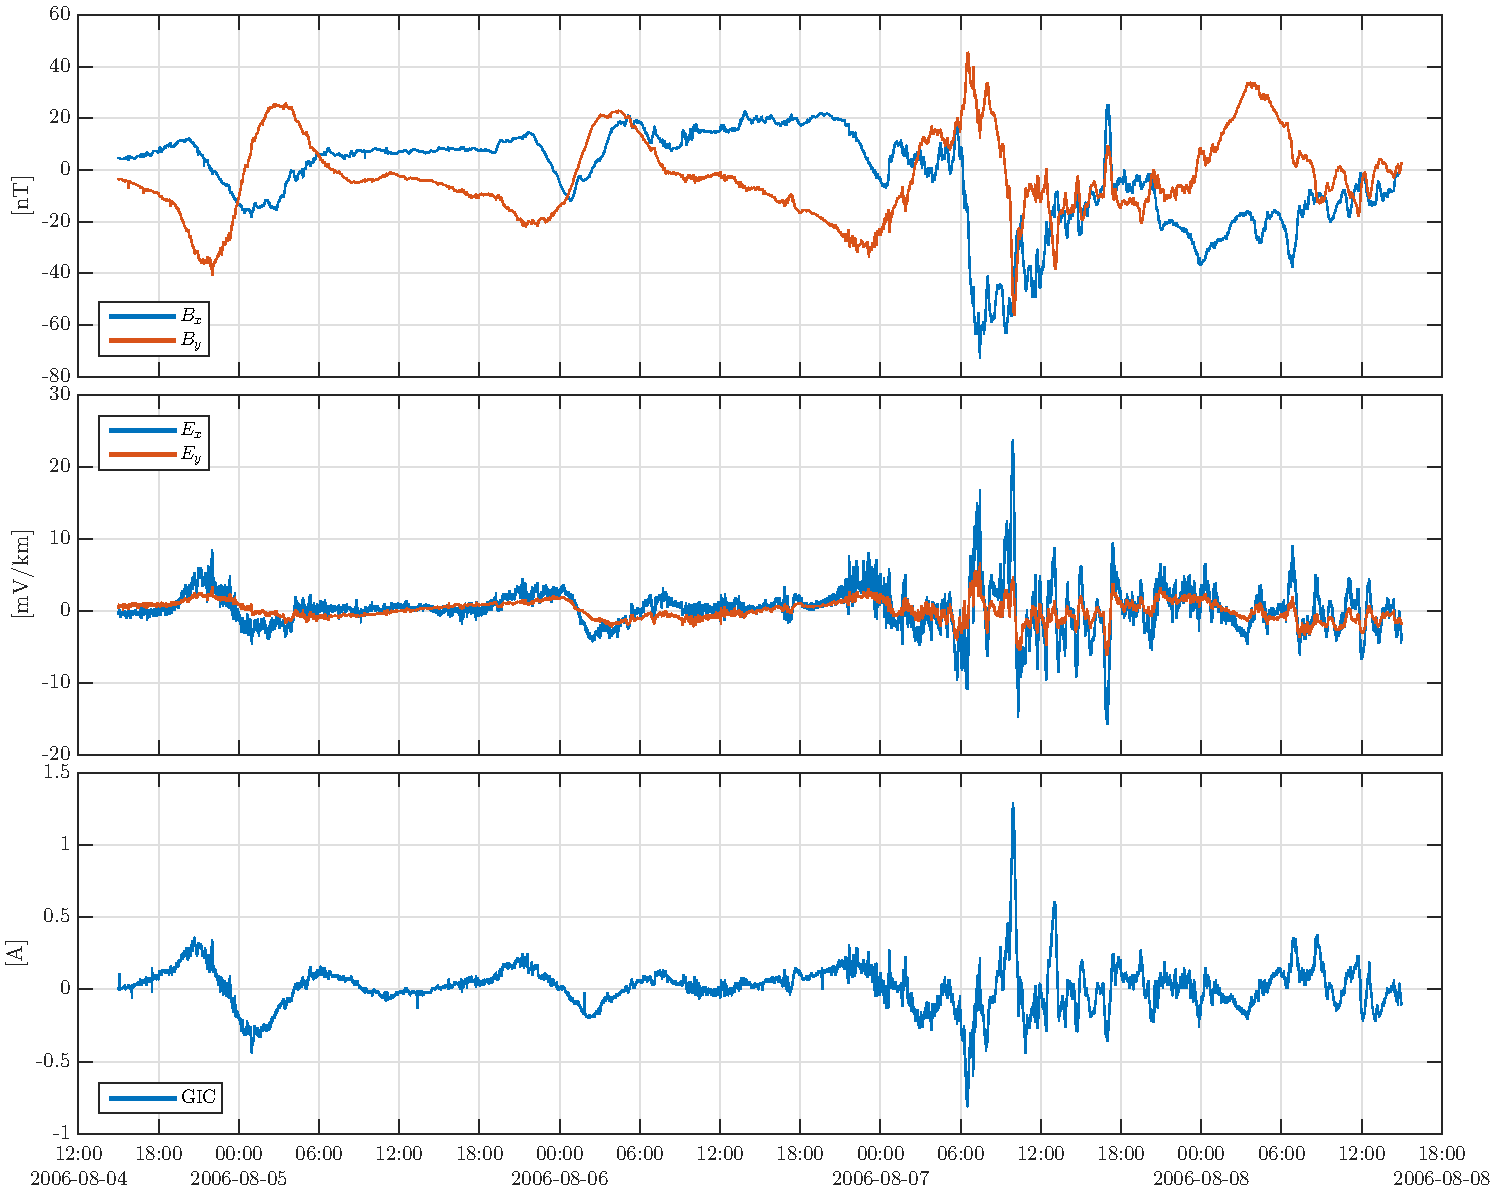
\includegraphics[width=\textwidth]{figures/plot_raw_All_20060805.pdf}
\caption{(Top) One-second-cadence geomagnetic field measured at the Memanbetsu Magnetic Observatory (MMB). (Middle) One-second-cadence geoelectric field measured at the Memanbetsu Magnetic Observatory (MMB) $\sim$10 km from the Memanbetsu substation. (Bottom) One-second-cadence GIC measurements measured in a grounded neutral point of a Y-connected three-phase transformer connected to a 187 kV bus at the Memanbetsu substation of the Hokkaido Power Co. The subscripts $x$ and $y$ correspond to Geographic North and East, respectively.}
\label{sample}
\end{figure}

\begin{figure}[h]
\centering
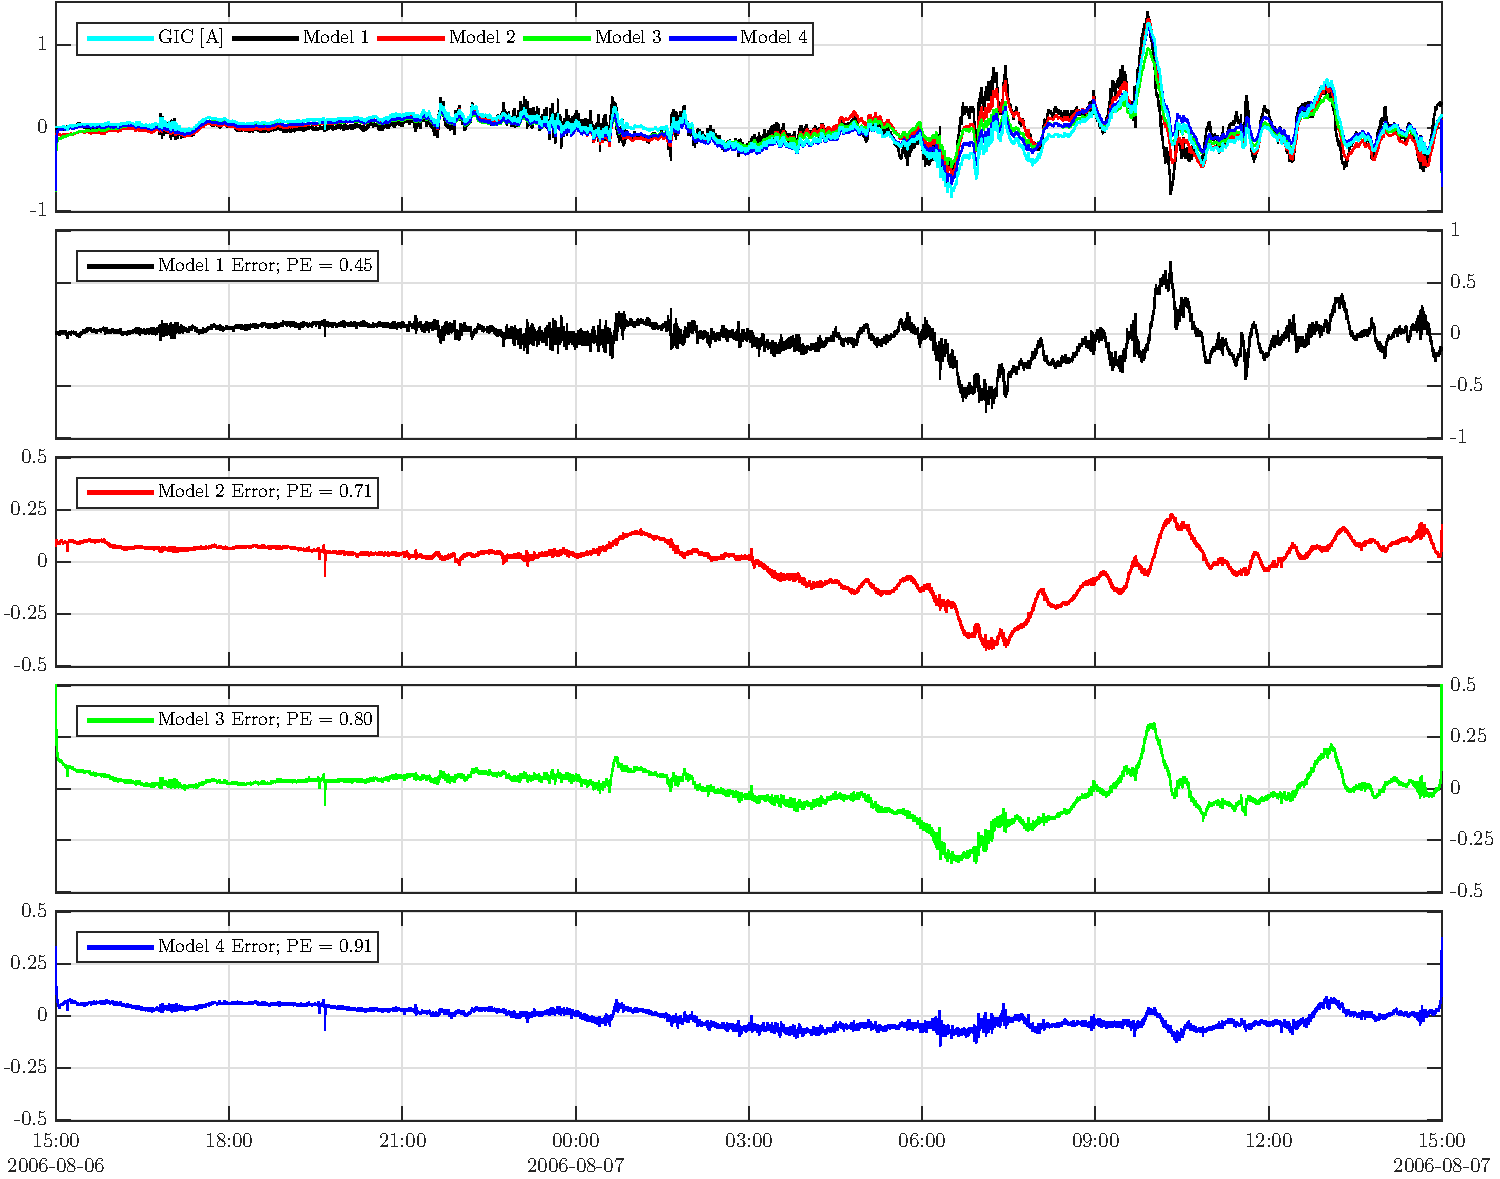
\includegraphics[width=\textwidth]{figures/plot_model_predictions-MeanModel-20060806T150000.pdf}
\caption{Out-of-sample model predictions (top) and predictions errors for a 1-day interval. Note that the scales for Models 2-4 differ from that for Model 1 so that the error amplitudes for Models 2-4 appear larger than that of Model 1 by a factor of 2.}
\label{predictions}
\end{figure}

\begin{figure}[h]
\centering
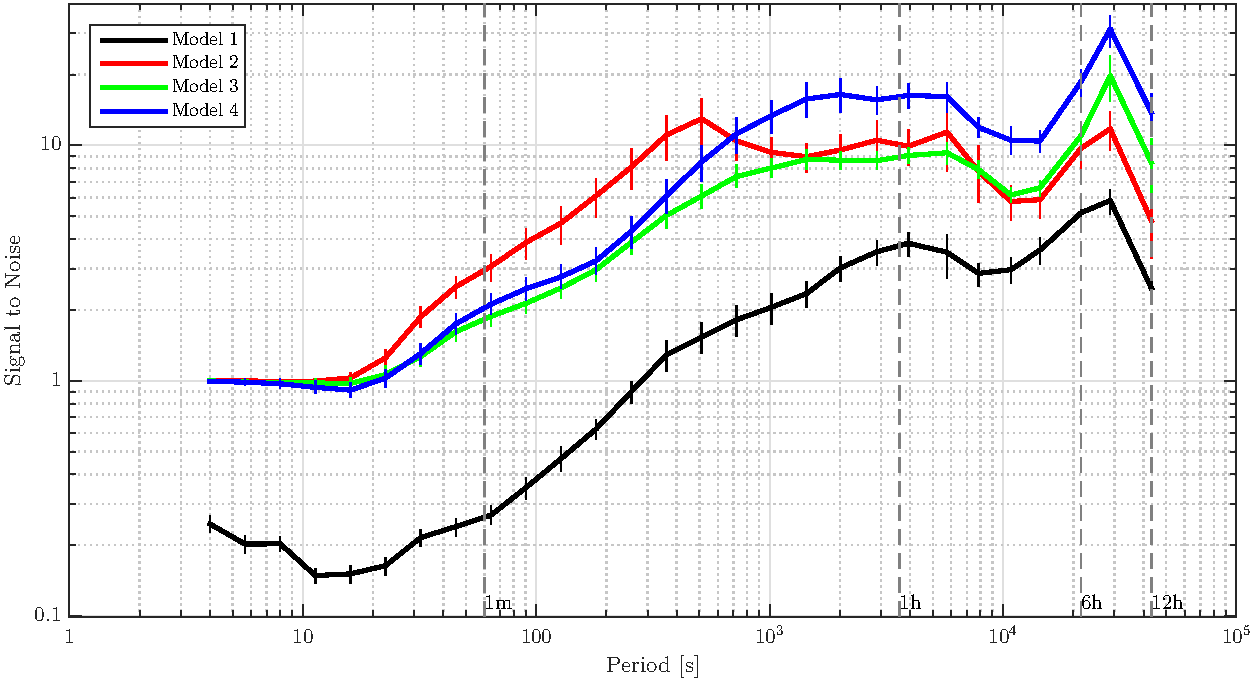
\includegraphics[width=\textwidth]{figures/plot_model_summary_SN-options-1.pdf}
\caption{Out-of-sample signal-to-noise ratios at the evaluation frequencies for the four models.}
\label{SN}
\end{figure}

\begin{figure}[h]
\centering
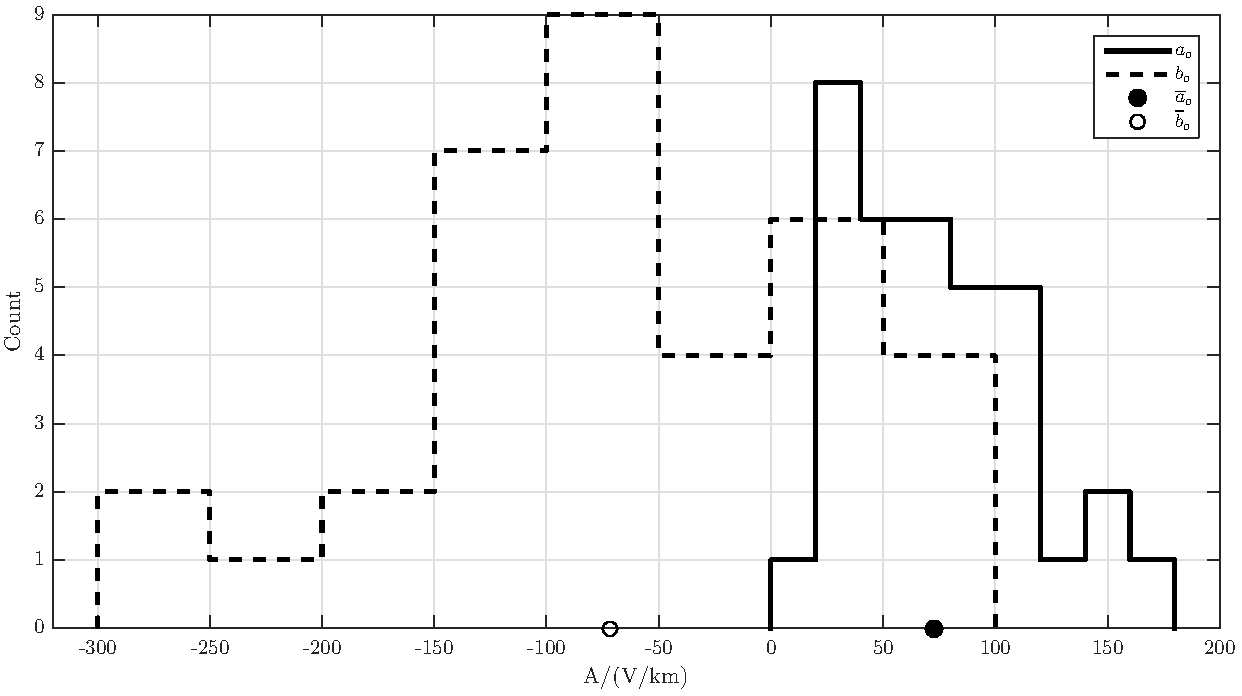
\includegraphics[width=\textwidth]{figures/plot_model_summary_aobo_histograms-options-1.pdf}
\caption{Distribution of parameters in Model 1. Each set of parameters was computed 35 times using one day of 1-second cadence data. The circle/dot on the horizontal axis indicates the average of each histogram: $a_o$ = 71.9 A/(V/km) and $b_o$ = -70.0 A/(V/km).}
\label{histogram}
\end{figure}

\begin{figure}[h]
\centering
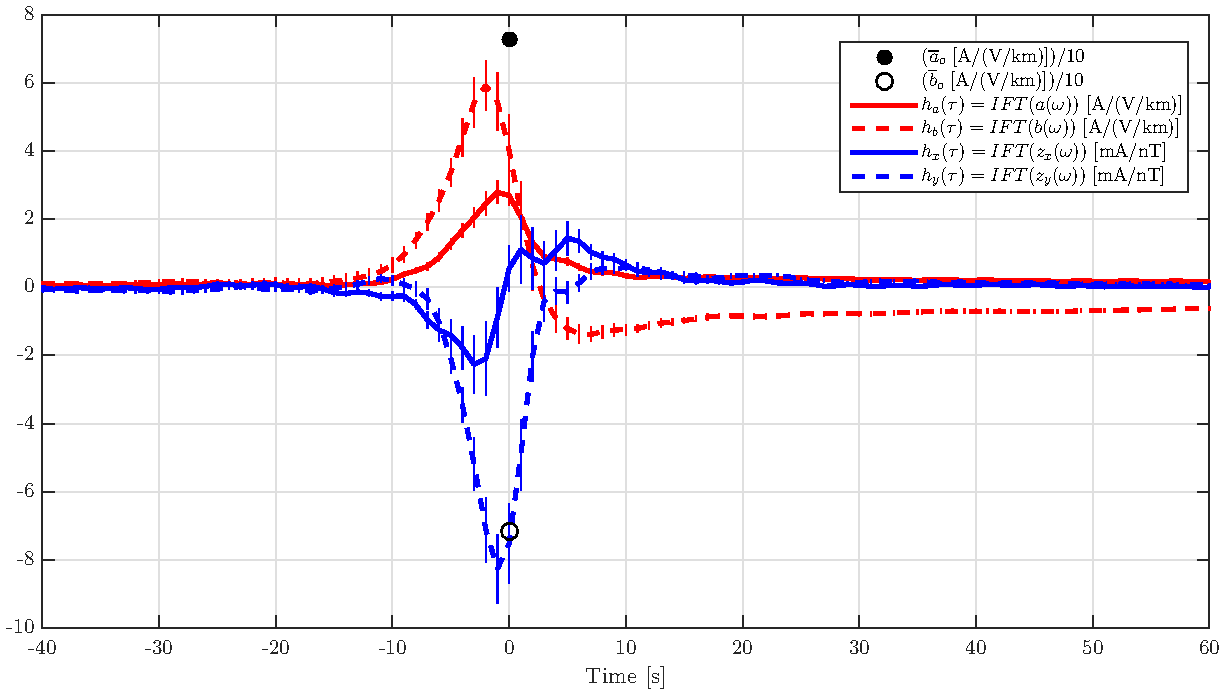
\includegraphics[width=\textwidth]{figures/plot_model_summary_H-options-1.pdf}
\caption{Impulse responses for Models 1, 2, and 4. The circles at $t = 0$ correspond to the impulse response for Model 1; the red/blue lines are the impulse responses for Model 2 and 4. The values of $a_o$ and $b_o$ have been scaled by a factor of 10 for readability.}
\label{H}
\end{figure}

\begin{figure}[h]
\centering
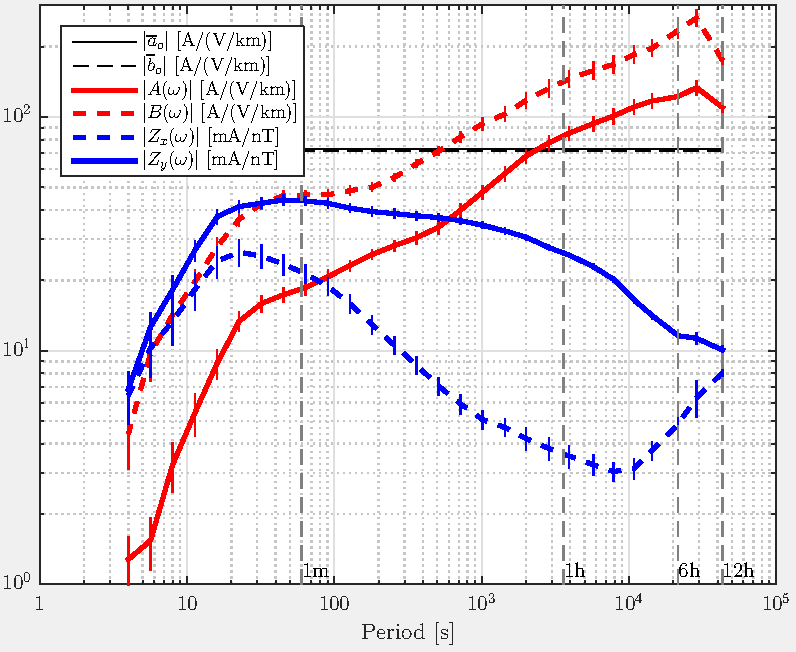
\includegraphics[width=\textwidth]{figures/plot_model_summary_Z-options-1.pdf}
\caption{Frequency domain transfer functions for Models 1-3, 2, and 4. The frequency domain transfer functions for $a_o$ and $b_o$ in Model~1 are constant and equal to $a_o$ and $b_o$.}
\label{Z}
\end{figure}

\begin{figure}[h]
\centering
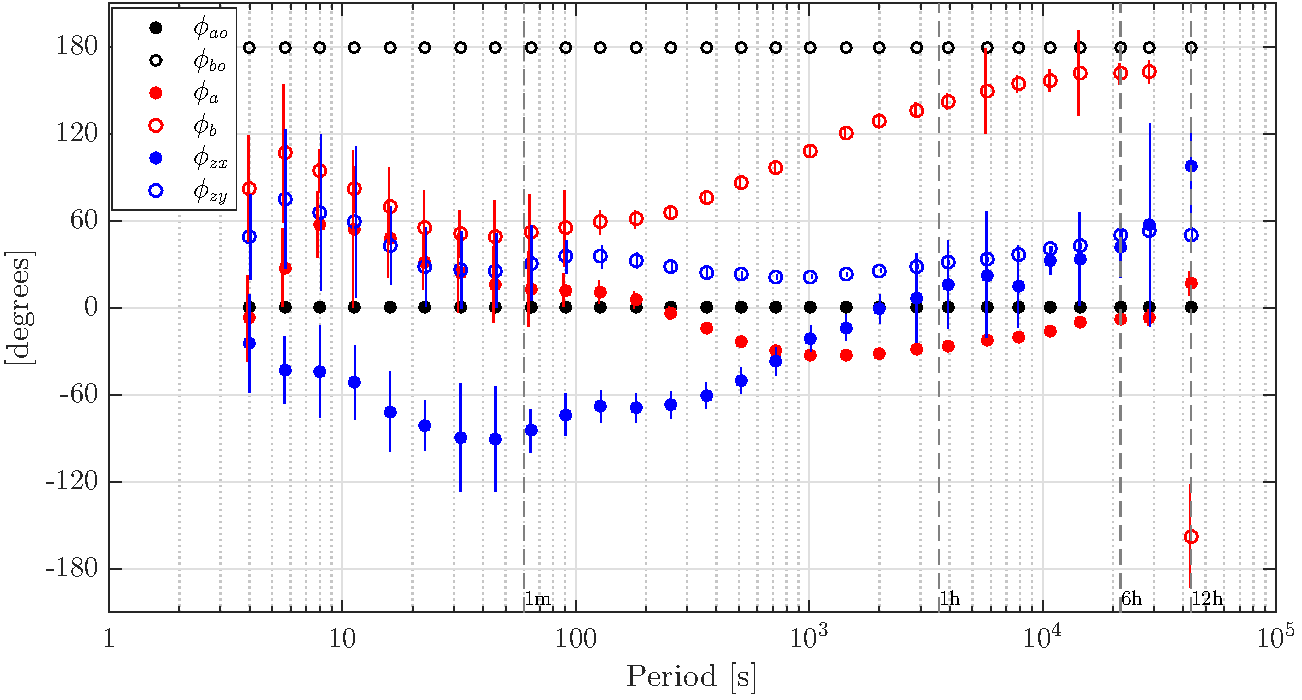
\includegraphics[width=\textwidth]{figures/plot_model_summary_Phi-options-1.pdf}
\caption{Frequency domain phase values for Models 1, 2, and 4. The phase for $a_o$ and $b_o$ in Model~1 are constant and equal to zero.}
\label{Phi}
\end{figure}

\clearpage

\appendix
\section{Appendix}

%Data from 2001-2011 have been used by ~\cite{Fujii2015} to estimate the magnetotelluric impedance at the site.

In the body of the work, a basic ordinary least squares method was used to compute transfer functions. Of course, there are many problems that one must address before the parameter estimates from a linear regression model can be used for a physical interpretation because the estimates may be biased, have high uncertainty, and be sensitive to outliers. In addition, to make inferences about ground conductivity, corrections must be made for distortion effects and violations of the plane wave assumption \citep{Simpson2005}.

Many robust alternatives to the basic least-squares for the calculation of transfer functions have been proposed and are strongly advocated by their developers to reduce uncertainty and sensitivity to outliers. For example, \cite{Egbert2011} notes that the least-squares method often fails and \cite{Chave1987} that failures are sometimes spectacular but more often insidious. However, ~\cite{Chave2017} has noted that the commonly used robust regression models are also problematic because the error model assumed for the calculation of robust transfer functions is often invalid due to the pervasiveness of non-gaussian residuals, and as a result it is not unconditionally unbiased.

There are also many approaches that are taken in pre-processing the data before regression is performed, for example, windowing in the time domain prior to the calculation of the fourier transform, windowing in the frequency domain to down-weight values far from the evaluation frequency or to down-weight frequencies that have low coherence, weighting values by an empirically estimated variance, pre-whitening, and using multi-taper methods to estimate spectra.

In general, the approach taken in the MT literature is to select a given variant of least squares and a set of pre-processing steps and to report the transfer functions along with an uncertainty (several approaches to estimating uncertainty exist as well). Absent an understanding of which particular regression alternative to use, the appropriate pre-processing approach, and the appropriate uncertainty estimate method, and an understanding of the appropriate adjustable parameters of each option and how they interact, the approach taken here is to investigate the influence of a few of the common regression alternatives, pre-processing steps, and stack-averaging methods on the transfer function estimate. 

The primary conclusion is that different methods generally give the statistically similar results in both the prediction metrics and parameter estimates except when the signal to noise ratio is low (below approximately $30$ seconds). Although parameter estimates were plotted below $30$ seconds because they were a part of the prediction models and they do contribute somewhat to the prediction efficiency, the estimates should be regarded as highly uncertain due to large error bars and a large sensitivity to the method used to calculate them.

The various tests that were performed to determine the influence of each method are summarized below and the associated results are shown in Figures~\ref{a_variations}-~\ref{b_variations}.

\begin{enumerate}

\item Robust regression was used instead of linear regression when computing the transfer function estimates at each $\omega_e$ (using a custom implementation with the $\psi$-function referenced in the next item and also using the \texttt{robustfit} function in MATLAB with either the bi-square and Huber weighting options). The motivation for the use of robust regression is to reduce the influence of outliers on the parameter estimates; ordinary least squares parameter estimates have a high sensitivity to outliers. When using robust regression, PEs and MSEs shown in Table~1 were the same to two decimal places and the confidence intervals were smaller by $\sim 2$\%. Figures~\ref{a_variations}-~\ref{b_variations} shows that the robust and used method give near identical estimates to the least square regression estimates.

\item Each 1-day segment was pre-whitened prior to calculation of the transfer functions in order to reduce the spectral range and to remove long-period drifts. This was done by computing the pre-whitening filter using a 10th-order Yule-Walker filter using $E_y$ for Model~2 and $B_x$ for Model~4 and applying this filter to all time series used in the calculation of the transfer function. The out-of-sample PEs were the same to within two decimal places and the MSE ratios varied by $0.05$.  Figures~\ref{a_variations}-~\ref{b_variations} show that pre-whitening has a larger impact on the estimates than robust regression.

\item A Parzen window was used to weight the fourier-transformed values instead of a rectangular window. This reduces the influence of values used in the transfer function parameter estimate as a function of distance from the evaluation frequency. The out-of-sample PEs for Model 3 and Model 4 were higher by $0.02$ and $0.01$, respectively and the MSE ratios for Models 3 and 4 were higher by $0.4$ and $0.6$, respectively. Figures~\ref{a_variations}-~\ref{b_variations} show that the pre-whitening has about the same amount of influence as the use of a Parzen window.

\item Five methods for averaging were used to compute magnitudes at each evaluation frequency of a complex-valued model parameter $p(D)$, where $D$ is estimate made using a 1-day of data. If $u(D)$ and $v(D)$ are the real and imaginary phase values for Models 2-4, then the $|p|$ was calculated as: (1) $|\text{mean}(u)+i\text{mean}(v)|$ (the method used), (2) $\text{mean}(|p|)$, (3) $|\text{median}(u)+i\text{median}(v)|$, (4) $\text{median}(|p|)$, and (5) $\text{mloc}(u) + i\text{mloc}(v)$, where the function $\text{mloc}$ is the Huber M-estimator \citep{Huber2011} with $\psi(x)=x$ for $|x|<1.5$ and $\psi(x) = 1.5$ for $x>1.5$ and $\psi(x) = -1.5$ for $x<-1.5$ (the \texttt{mlochuber} function in LIBRA \citep{Verboven2010} was used for the calculation). The out-of-sample PEs varied by $\pm 0.01$ and MSE ratios shown in Table~1 differed by at most $0.03$. Neither averaging method was yielded consistently higher or lower values. Figures~\ref{a_variations}-~\ref{b_variations} shows that most of the sensitivity is below $T=20$ s, as expected, due to the signal-to-noise being near equal to 1 below this period.

\end{enumerate}

Several addition experiments were performed that we summarize with text only.

\begin{enumerate}
\item Instead computing an average transfer function by a simple average of the 35 transfer functions, weighted averages were considered. The weighting included using the in-sample coherence or prediction efficiency (ad-hoc approaches to give higher weight to better fitting intervals) and weighting the collection of values used to compute the model parameters at a given evaluation frequency by a smoothed estimate of the PSD of the predictand (to account for the fact that the signal to noise ratio depends on frequency as evident in ~\ref{SN} and noted by \citep{Egbert1997}; accounting for this can reduce the variance in the parameter estimates). An approach that is more similar to that used in \citep{Egbert1997} was also used - prior to regression, the the values were weighted with a weight that is inversely proportional to an estimate of of the spectra of the vector magnitude of the input. 

\item At a given frequency, we have found that there is a correlation between the parameter estimate and the PSD of the input, output, and prediction error that varies between +0.6 and -0.2, which is one of the many ways in which the data violate the assumptions for OLS estimates to be the best linear unbiased estimator. To determine how this violation could effect the parameter estimates, at each frequency, the top 17 and lowest 18 transfer functions were averaged and plotted as a function of frequency. The parameter estimates from the high input PSD intervals tended to be higher, but within the range of the displayed error bars.

\item Instead of calculating 35 transfer functions and then averaging, compute one transfer function - for each evaluation frequency, combine the 35 fourier spectra values near that evaluation frequency and use them for one regression.  
\end{enumerate}

%In all cases, the parameter estimates below $\sim 20$ seconds using the alternative methods were consistently lower, but the offset was of magnitude that was similar to the variation observed between the alternative methods. The largest variations were found in relative to the method used to averaging the 35 transfer functions. In addition, how the averages were made when computing the magnitudes mattered - if the magnitudes at a given frequency were calculated by taking the modulus of the mean of the 35 real and mean of the 35 imaginary components vs the mean of the modulus of the 35 transfer functions. The same was true for the median.

\clearpage

\begin{figure}[h]
\begin{minipage}[t]{.48\linewidth}
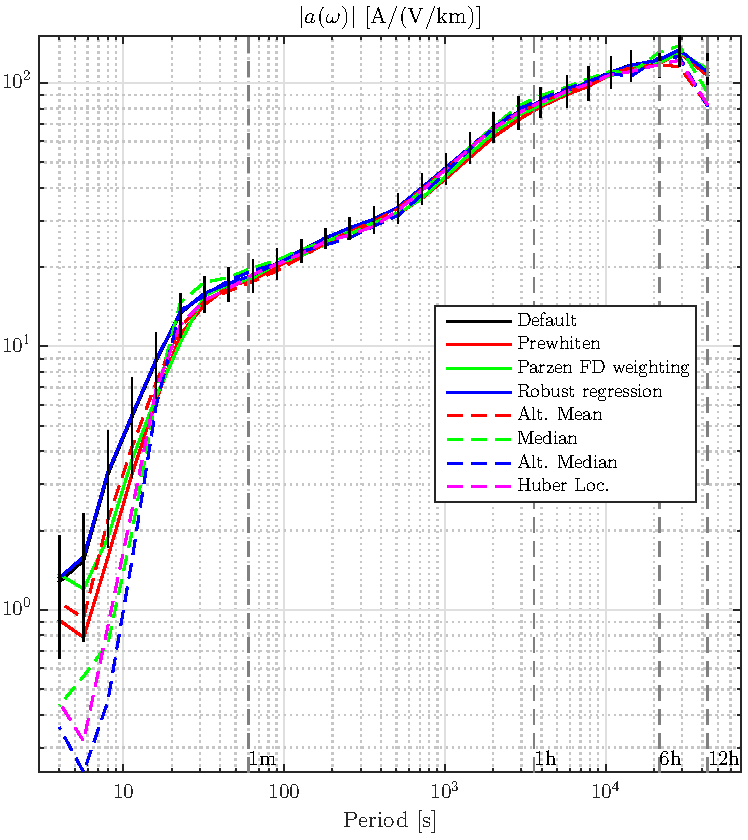
\includegraphics[width=\textwidth]{figures/plot_options_comparison_a.pdf}
\label{plot_options_comparison_a}
\end{minipage}
\begin{minipage}[t]{.48\linewidth}
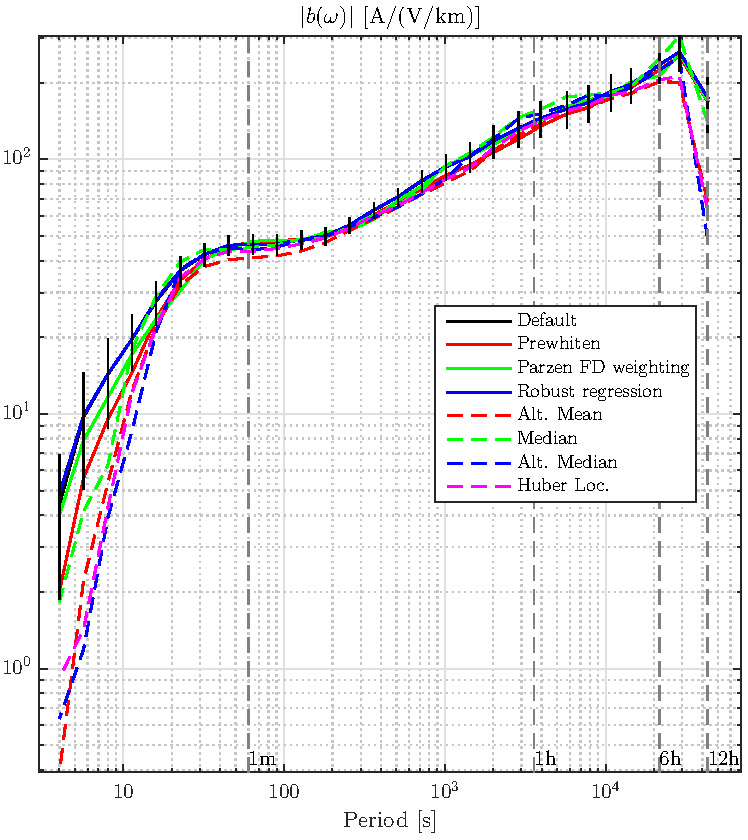
\includegraphics[width=\textwidth]{figures/plot_options_comparison_b.pdf}
\end{minipage}
\begin{minipage}[t]{.48\linewidth}
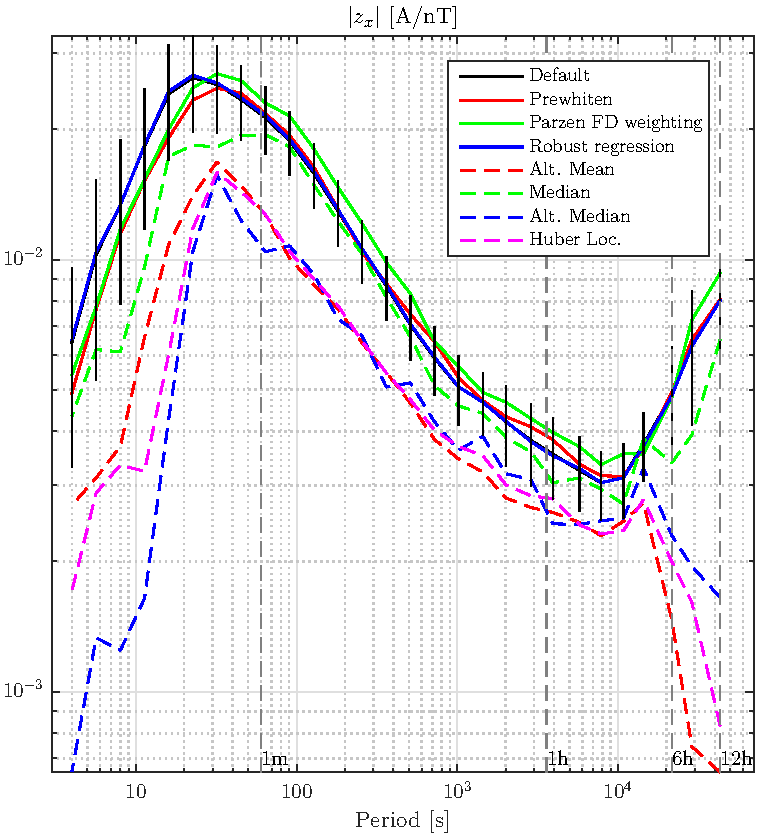
\includegraphics[width=\textwidth]{figures/plot_options_comparison_zx.pdf}
\label{plot_options_comparison_a}
\end{minipage}
\begin{minipage}[t]{.48\linewidth}
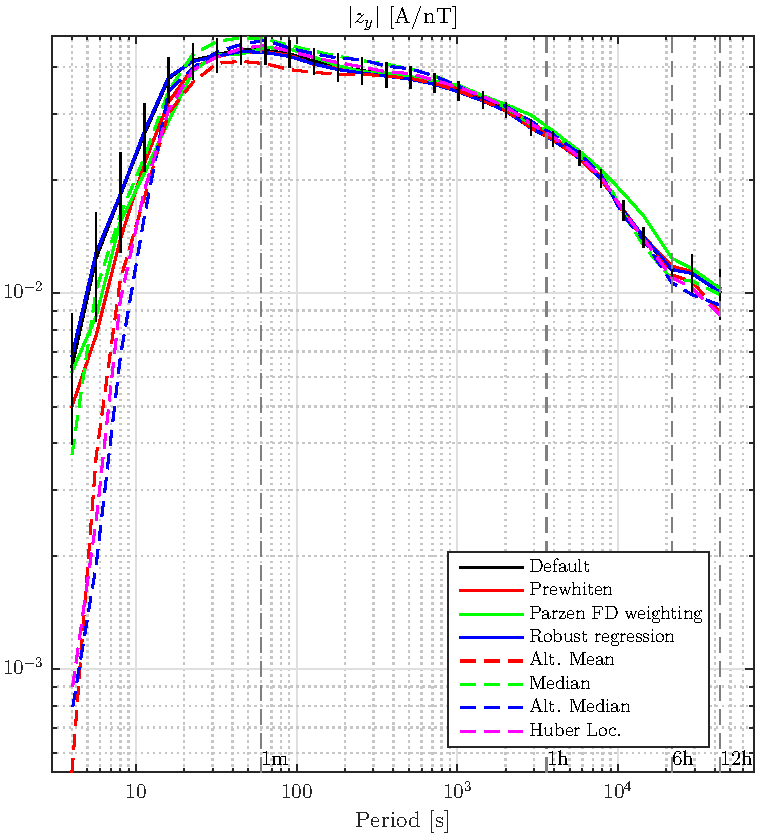
\includegraphics[width=\textwidth]{figures/plot_options_comparison_zy.pdf}
\end{minipage}

\end{figure}

\clearpage

\bibliography{paper.bib}

% Please use ONLY \citet and \citep for reference citations.
% DO NOT use other cite commands (e.g., \cite, \citeyear, \nocite, \citealp, etc.).
%% Example \citet and \citep:
%  ...as shown by \citet{Boug10}, \citet{Buiz07}, \citet{Fra10},
%  \citet{Ghel00}, and \citet{Leit74}.

%  ...as shown by \citep{Boug10}, \citep{Buiz07}, \citep{Fra10},
%  \citep{Ghel00, Leit74}.

\end{document}



More Information and Advice:

%% ------------------------------------------------------------------------ %%
%
%  SECTION HEADS
%
%% ------------------------------------------------------------------------ %%

% Capitalize the first letter of each word (except for
% prepositions, conjunctions, and articles that are
% three or fewer letters).

% AGU follows standard outline style; therefore, there cannot be a section 1 without
% a section 2, or a section 2.3.1 without a section 2.3.2.
% Please make sure your section numbers are balanced.
% ---------------
% Level 1 head
%
% Use the \section{} command to identify level 1 heads;
% type the appropriate head wording between the curly
% brackets, as shown below.
%
%An example:
%\section{Level 1 Head: Introduction}
%
% ---------------
% Level 2 head
%
% Use the \subsection{} command to identify level 2 heads.
%An example:
%\subsection{Level 2 Head}
%
% ---------------
% Level 3 head
%
% Use the \subsubsection{} command to identify level 3 heads
%An example:
%\subsubsection{Level 3 Head}
%
%---------------
% Level 4 head
%
% Use the \subsubsubsection{} command to identify level 3 heads
% An example:
%\subsubsubsection{Level 4 Head} An example.
%
%% ------------------------------------------------------------------------ %%
%
%  IN-TEXT LISTS
%
%% ------------------------------------------------------------------------ %%
%
% Do not use bulleted lists; enumerated lists are okay.
% \begin{enumerate}
% \item
% \item
% \item
% \end{enumerate}
%
%% ------------------------------------------------------------------------ %%
%
%  EQUATIONS
%
%% ------------------------------------------------------------------------ %%

% Single-line equations are centered.
% Equation arrays will appear left-aligned.

Math coded inside display math mode \[ ...\]
 will not be numbered, e.g.,:
 \[ x^2=y^2 + z^2\]

 Math coded inside \begin{equation} and \end{equation} will
 be automatically numbered, e.g.,:
 \begin{equation}
 x^2=y^2 + z^2
 \end{equation}


% To create multiline equations, use the
% \begin{eqnarray} and \end{eqnarray} environment
% as demonstrated below.
\begin{eqnarray}
  x_{1} & = & (x - x_{0}) \cos \Theta \nonumber \\
        && + (y - y_{0}) \sin \Theta  \nonumber \\
  y_{1} & = & -(x - x_{0}) \sin \Theta \nonumber \\
        && + (y - y_{0}) \cos \Theta.
\end{eqnarray}

%If you don't want an equation number, use the star form:
%\begin{eqnarray*}...\end{eqnarray*}

% Break each line at a sign of operation
% (+, -, etc.) if possible, with the sign of operation
% on the new line.

% Indent second and subsequent lines to align with
% the first character following the equal sign on the
% first line.

% Use an \hspace{} command to insert horizontal space
% into your equation if necessary. Place an appropriate
% unit of measure between the curly braces, e.g.
% \hspace{1in}; you may have to experiment to achieve
% the correct amount of space.


%% ------------------------------------------------------------------------ %%
%
%  EQUATION NUMBERING: COUNTER
%
%% ------------------------------------------------------------------------ %%

% You may change equation numbering by resetting
% the equation counter or by explicitly numbering
% an equation.

% To explicitly number an equation, type \eqnum{}
% (with the desired number between the brackets)
% after the \begin{equation} or \begin{eqnarray}
% command.  The \eqnum{} command will affect only
% the equation it appears with; LaTeX will number
% any equations appearing later in the manuscript
% according to the equation counter.
%

% If you have a multiline equation that needs only
% one equation number, use a \nonumber command in
% front of the double backslashes (\\) as shown in
% the multiline equation above.

% If you are using line numbers, remember to surround
% equations with \begin{linenomath*}...\end{linenomath*}

%  To add line numbers to lines in equations:
%  \begin{linenomath*}
%  \begin{equation}
%  \end{equation}
%  \end{linenomath*}
